
\documentclass[a4paper,11pt]{article}
\usepackage[a4paper, margin=8em]{geometry}

% usa i pacchetti per la scrittura in italiano
\usepackage[french,italian]{babel}
\usepackage[T1]{fontenc}
\usepackage[utf8]{inputenc}
\frenchspacing 

% usa i pacchetti per la formattazione matematica
\usepackage{amsmath, amssymb, amsthm, amsfonts}

% usa altri pacchetti
\usepackage{gensymb}
\usepackage{hyperref}
\usepackage{standalone}

\usepackage{colortbl}

\usepackage{xstring}
\usepackage{karnaugh-map}

% imposta il titolo
\title{Computer Architectures notes}
\author{Luca Seggiani}
\date{2026}

% imposta lo stile
% usa helvetica
\usepackage[scaled]{helvet}
% usa palatino
\usepackage{palatino}
% usa un font monospazio guardabile
\usepackage{lmodern}

\renewcommand{\rmdefault}{ppl}
\renewcommand{\sfdefault}{phv}
\renewcommand{\ttdefault}{lmtt}

% circuiti
\usepackage{circuitikz}
\usetikzlibrary{babel}

% testo cerchiato
\newcommand*\circled[1]{\tikz[baseline=(char.base)]{
            \node[shape=circle,draw,inner sep=2pt] (char) {#1};}}

% disponi il titolo
\makeatletter
\renewcommand{\maketitle} {
	\begin{center} 
		\begin{minipage}[t]{.8\textwidth}
			\textsf{\huge\bfseries \@title} 
		\end{minipage}%
		\begin{minipage}[t]{.2\textwidth}
			\raggedleft \vspace{-1.65em}
			\textsf{\small \@author} \vfill
			\textsf{\small \@date}
		\end{minipage}
		\par
	\end{center}

	\thispagestyle{empty}
	\pagestyle{fancy}
}
\makeatother

% disponi teoremi
\usepackage{tcolorbox}
\newtcolorbox[auto counter, number within=section]{theorem}[2][]{%
	colback=blue!10, 
	colframe=blue!40!black, 
	sharp corners=northwest,
	fonttitle=\sffamily\bfseries, 
	title=Theorem~\thetcbcounter: #2, 
	#1
}

% disponi definizioni
\newtcolorbox[auto counter, number within=section]{definition}[2][]{%
	colback=red!10,
	colframe=red!40!black,
	sharp corners=northwest,
	fonttitle=\sffamily\bfseries,
	title=Definition~\thetcbcounter: #2,
	#1
}

% disponi codice
\usepackage{listings}
\usepackage[table]{xcolor}

\definecolor{codegreen}{rgb}{0,0.6,0}
\definecolor{codegray}{rgb}{0.5,0.5,0.5}
\definecolor{codepurple}{rgb}{0.58,0,0.82}
\definecolor{backcolour}{rgb}{0.95,0.95,0.92}

\lstdefinestyle{codestyle}{
		backgroundcolor=\color{black!5}, 
		commentstyle=\color{codegreen},
		keywordstyle=\bfseries\color{magenta},
		numberstyle=\sffamily\tiny\color{black!60},
		stringstyle=\color{green!50!black},
		basicstyle=\ttfamily\footnotesize,
		breakatwhitespace=false,         
		breaklines=true,                 
		captionpos=b,                    
		keepspaces=true,                 
		numbers=left,                    
		numbersep=5pt,                  
		showspaces=false,                
		showstringspaces=false,
		showtabs=false,                  
		tabsize=2
}

\lstdefinestyle{shellstyle}{
		backgroundcolor=\color{black!5}, 
		basicstyle=\ttfamily\footnotesize\color{black}, 
		commentstyle=\color{black}, 
		keywordstyle=\color{black},
		numberstyle=\color{black!5},
		stringstyle=\color{black}, 
		showspaces=false,
		showstringspaces=false, 
		showtabs=false, 
		tabsize=2, 
		numbers=none, 
		breaklines=true
}

\lstdefinelanguage{x86}{ 
  keywords={AAA, AAD, AAM, AAS, ADC, ADCB, ADCW, ADCL, ADD, ADDB, ADDW, ADDL, AND, ANDB, ANDW, ANDL,
        ARPL, BOUND, BSF, BSFL, BSFW, BSR, BSRL, BSRW, BSWAP, BT, BTC, BTCB, BTCW, BTCL, BTR, 
        BTRB, BTRW, BTRL, BTS, BTSB, BTSW, BTSL, CALL, CBW, CDQ, CLC, CLD, CLI, CLTS, CMC, CMP,
        CMPB, CMPW, CMPL, CMPS, CMPSB, CMPSD, CMPSW, CMPXCHG, CMPXCHGB, CMPXCHGW, CMPXCHGL,
        CMPXCHG8B, CPUID, CWDE, DAA, DAS, DEC, DECB, DECW, DECL, DIV, DIVB, DIVW, DIVL, ENTER,
        HLT, IDIV, IDIVB, IDIVW, IDIVL, IMUL, IMULB, IMULW, IMULL, IN, INB, INW, INL, INC, INCB,
        INCW, INCL, INS, INSB, INSD, INSW, INT, INT3, INTO, INVD, INVLPG, IRET, IRETD, JA, JAE,
        JB, JBE, JC, JCXZ, JE, JECXZ, JG, JGE, JL, JLE, JMP, JNA, JNAE, JNB, JNBE, JNC, JNE, JNG,
        JNGE, JNL, JNLE, JNO, JNP, JNS, JNZ, JO, JP, JPE, JPO, JS, JZ, LAHF, LAR, LCALL, LDS,
        LEA, LEAVE, LES, LFS, LGDT, LGS, LIDT, LMSW, LOCK, LODSB, LODSD, LODSW, LOOP, LOOPE,
        LOOPNE, LSL, LSS, LTR, MOV, MOVB, MOVW, MOVL, MOVSB, MOVSD, MOVSW, MOVSX, MOVSXB,
        MOVSXW, MOVSXL, MOVZX, MOVZXB, MOVZXW, MOVZXL, MUL, MULB, MULW, MULL, NEG, NEGB, NEGW,
        NEGL, NOP, NOT, NOTB, NOTW, NOTL, OR, ORB, ORW, ORL, OUT, OUTB, OUTW, OUTL, OUTSB, OUTSD,
        OUTSW, POP, POPL, POPW, POPB, POPA, POPAD, POPF, POPFD, PUSH, PUSHL, PUSHW, PUSHB, PUSHA, 
        RCLL, RCR, RCRB, RCRW, RCRL, RDMSR, RDPMC, RDTSC, REP, REPE, REPNE, RET, ROL, ROLB, ROLW,
        ROLL, ROR, RORB, RORW, RORL, SAHF, SAL, SALB, SALW, SALL, SAR, SARB, SARW, SARL, SBB,
        SBBB, SBBW, SBBL, SCASB, SCASD, SCASW, SETA, SETAE, SETB, SETBE, SETC, SETE, SETG, SETGE,
        SETL, SETLE, SETNA, SETNAE, SETNB, SETNBE, SETNC, SETNE, SETNG, SETNGE, SETNL, SETNLE,
        SETNO, SETNP, SETNS, SETNZ, SETO, SETP, SETPE, SETPO, SETS, SETZ, SGDT, SHL, SHLB, SHLW,
        SHLL, SHLD, SHR, SHRB, SHRW, SHRL, SHRD, SIDT, SLDT, SMSW, STC, STD, STI, STOSB, STOSD,
        STOSW, STR, SUB, SUBB, SUBW, SUBL, TEST, TESTB, TESTW, TESTL, VERR, VERW, WAIT, WBINVD,
        XADD, XADDB, XADDW, XADDL, XCHG, XCHGB, XCHGW, XCHGL, XLAT, XLATB, XOR, XORB, XORW, XORL},
  keywordstyle=\color{blue}\bfseries,
  ndkeywordstyle=\color{darkgray}\bfseries,
  identifierstyle=\color{black},
  sensitive=false,
  comment=[l]{\#},
  morecomment=[s]{/*}{*/},
  commentstyle=\color{purple}\ttfamily,
  stringstyle=\color{red}\ttfamily,
  morestring=[b]',
  morestring=[b]"
}

\lstdefinelanguage{riscv}{
  keywords={
    LUI, AUIPC,
    JAL, JALR,
    BEQ, BNE, BLT, BGE, BLTU, BGEU,
    LB, LH, LW, LBU, LHU, LD,
    SB, SH, SW, SD,
    ADDI, SLTI, SLTIU, XORI, ORI, ANDI,
    SLLI, SRLI, SRAI,
    ADD, SUB, SLL, SLT, SLTU, XOR, SRL, SRA, OR, AND,
    ADDIW, SLLIW, SRLIW, SRAIW,
    ADDW, SUBW, SLLW, SRLW, SRAW,
    MUL, MULH, MULHSU, MULHU, DIV, DIVU, REM, REMU,
    MULW, DIVW, DIVUW, REMW, REMUW,
    LR.W, SC.W, AMOSWAP.W, AMOADD.W, AMOXOR.W,
    AMOAND.W, AMOOR.W, AMOMIN.W, AMOMAX.W,
    AMOMINU.W, AMOMAXU.W,
    LR.D, SC.D, AMOSWAP.D, AMOADD.D, AMOXOR.D,
    AMOAND.D, AMOOR.D, AMOMIN.D, AMOMAX.D,
    AMOMINU.D, AMOMAXU.D,
    FLW, FSW,
    FMADD.S, FMSUB.S, FNMSUB.S, FNMADD.S,
    FADD.S, FSUB.S, FMUL.S, FDIV.S, FSQRT.S,
    FSGNJ.S, FSGNJN.S, FSGNJX.S,
    FMIN.S, FMAX.S,
    FCVT.W.S, FCVT.WU.S, FCVT.S.W, FCVT.S.WU,
    FMV.X.W, FMV.W.X,
    FEQ.S, FLT.S, FLE.S,
    FLD, FSD,
    FMADD.D, FMSUB.D, FNMSUB.D, FNMADD.D,
    FADD.D, FSUB.D, FMUL.D, FDIV.D, FSQRT.D,
    FSGNJ.D, FSGNJN.D, FSGNJX.D,
    FMIN.D, FMAX.D,
    FCVT.W.D, FCVT.WU.D, FCVT.D.W, FCVT.D.WU,
    FCVT.S.D, FCVT.D.S,
    FMV.X.D, FMV.D.X,
    FEQ.D, FLT.D, FLE.D,
    CSRRW, CSRRS, CSRRC,
    CSRRWI, CSRRSI, CSRRCI,
    FENCE.I,
    FENCE,
    ECALL, EBREAK,
    MRET, SRET, URET,
    WFI,
    SFENCE.VMA,
    NOP, LI, LA, MV,
    NOT, NEG, NEGW,
    SEQZ, SNEZ, SLTZ, SGTZ,
    BEQZ, BNEZ, BLEZ, BGEZ, BLTZ, BGTZ,
    BGT, BLE, BGTU, BLEU,
    J, JR, RET,
    CALL, TAIL,
    RDINSTRET, RDCYCLE, RDTIME,
    CSRR, CSRW, CSRS, CSRC,
    CSRWI, CSRSI, CSRCI
  },
  keywordstyle=\color{blue}\bfseries,
  ndkeywordstyle=\color{darkgray}\bfseries,
  identifierstyle=\color{black},
  sensitive=false,
  comment=[l]{\#},
  morecomment=[s]{/*}{*/},
  commentstyle=\color{purple}\ttfamily,
  stringstyle=\color{red}\ttfamily,
  morestring=[b]',
  morestring=[b]"
}

\lstdefinelanguage{arm}{
  keywords={
    ADC, ADD, AND, BIC, CMN, CMP, EOR, MOV, MVN,
    RSB, RSC, SBC, SUB, TST, TEQ,
    MLA, MLS, MUL, SMLAL, SMULL, UMLAL, UMULL,
    QADD, QSUB, QDADD, QDSUB,
    QADD16, QADD8, QASX, QSAX,
    QSUB16, QSUB8, QSAX, QSUBADDX,
    ASR, LSL, LSR, ROR, RRX,
    B, BL, BX, BLX,
    BXJ,
    BEQ, BNE, BCS, BHS, BCC, BLO,
    BMI, BPL, BVS, BVC,
    BHI, BLS, BGE, BLT, BGT, BLE,
    BAL,
    LDR, LDRB, LDRH, LDRSB, LDRSH,
    LDRD, LDM, LDMIA, LDMIB, LDMDA, LDMDB,
    LDRT, LDRBT, LDRHT, LDRSBT, LDRSHT,
    STR, STRB, STRH, STRD,
    STM, STMIA, STMIB, STMDA, STMDB,
    STRT, STRBT, STRHT,
    PUSH, POP,
    SWP, SWPB,
    REV, REV16, REVSH,
    BFC, BFI, BFXIL, SBFX, UBFX,
    CLZ,
    LDREX, LDREXB, LDREXH, LDREXD,
    STREX, STREXB, STREXH, STREXD,
    DMB, DSB, ISB,
    MCR, MCRR, MRC, MRRC,
    MRS, MSR,
    CPS, SETEND, SVC, BKPT,
    CLREX, WFE, WFI, SEV,
    YIELD, NOP,
    VLDR, VSTR,
    VMOV, VABS, VNEG,
    VADD, VSUB, VMUL, VDIV,
    VMLA, VMLS, VNMLA, VNMLS, VNMUL,
    VMAX, VMIN,
    VSQRT,
    VCMP, VCMPE,
    VCVT,
    VCLZ, VCLS,
    VAND, VORR, VEOR, VBIC, VMVN,
    VLD1, VLD2, VLD3, VLD4,
    VST1, VST2, VST3, VST4,
    ADR, ADCS, ADDS, SUBS, MOVS, ANDS, ORRS, EORS
  },
  keywordstyle=\color{blue}\bfseries,
  ndkeywordstyle=\color{darkgray}\bfseries,
  identifierstyle=\color{black},
  sensitive=false,
  comment=[l]{@},
  morecomment=[l]{;},
  morecomment=[s]{/*}{*/},
  commentstyle=\color{purple}\ttfamily,
  stringstyle=\color{red}\ttfamily,
  morestring=[b]',
  morestring=[b]"
}

\lstset{style=codestyle, language=C}

% disponi sezioni
\usepackage{titlesec}

\titleformat{\section}
	{\sffamily\Large\bfseries} 
	{\thesection}{1em}{} 
\titleformat{\subsection}
	{\sffamily\large\bfseries}   
	{\thesubsection}{1em}{} 
\titleformat{\subsubsection}
	{\sffamily\normalsize\bfseries} 
	{\thesubsubsection}{1em}{}

% tikz
\usepackage{tikz}

% float
\usepackage{float}

% grafici
\usepackage{pgfplots}
\pgfplotsset{width=10cm,compat=1.9}

% disponi alberi
\usepackage{forest}

\forestset{
	rectstyle/.style={
		for tree={rectangle,draw,font=\large\sffamily}
	},
	roundstyle/.style={
		for tree={circle,draw,font=\large}
	}
}

% disponi algoritmi
\usepackage{algorithm}
\usepackage{algorithmic}
\makeatletter
\renewcommand{\ALG@name}{Algorithm}
\makeatother

% disponi numeri di pagina
\usepackage{fancyhdr}
\fancyhf{} 
\fancyfoot[L]{\sffamily{\thepage}}

\makeatletter
\fancyhead[L]{\raisebox{1ex}[0pt][0pt]{\sffamily{\@title \ \@date}}} 
\fancyhead[R]{\raisebox{1ex}[0pt][0pt]{\sffamily{\@author}}}
\makeatother

\begin{document}
% sezione (data)
\section{Lesson 02-10-26}

% stili pagina
\thispagestyle{empty}
\pagestyle{fancy}

% testo
\subsection{Control hazards}

We know move on to discussing \textbf{control hazards}.
We explicitly ignored them until now as they are:
\begin{itemize}
	\item Slightly more complicated;
	\item Open up a world of possibilities for CPU optimizations.
\end{itemize}

They are due to branches (conditional and unconditional), which may change the PC after the following instruction has been fetched already.
In the case of conditional branches, the decision on whether the PC should be modified (branch taken) or not (branch untaken) can be taken even later.
In the basic RISC-V implementation, the PC is written with the target address (if the jump is taken) at the end of the EXE stage, i.e., 2 clock cycles after the IF of the branch.
This behavior delays the target instruction by two clock cycles.

\subsubsection{Stalling}

A possible solution is based on stalling the pipeline as soon as a branch instruction is detected (ID stage) by:
\begin{itemize}
	\item Deciding earlier whether the branch has to be taken or not;
	\item Computing earlier the new PC value.
\end{itemize}

This means that we make a temporary decision and continue loading the pipeline as if the branch wasn't there (or as if it was always taken, depending on the prediction).
If the branch does, in fact, get taken (or not taken) then we wasted clock cycles and have to flush the pipeline.
Otherwise, we win.

\subsubsection{Stalling with modified pipeline}

This clearly has an advantage in modifying the pipeline for early branch address computation (in the ID stage instead of the EX stage).

\begin{center}
	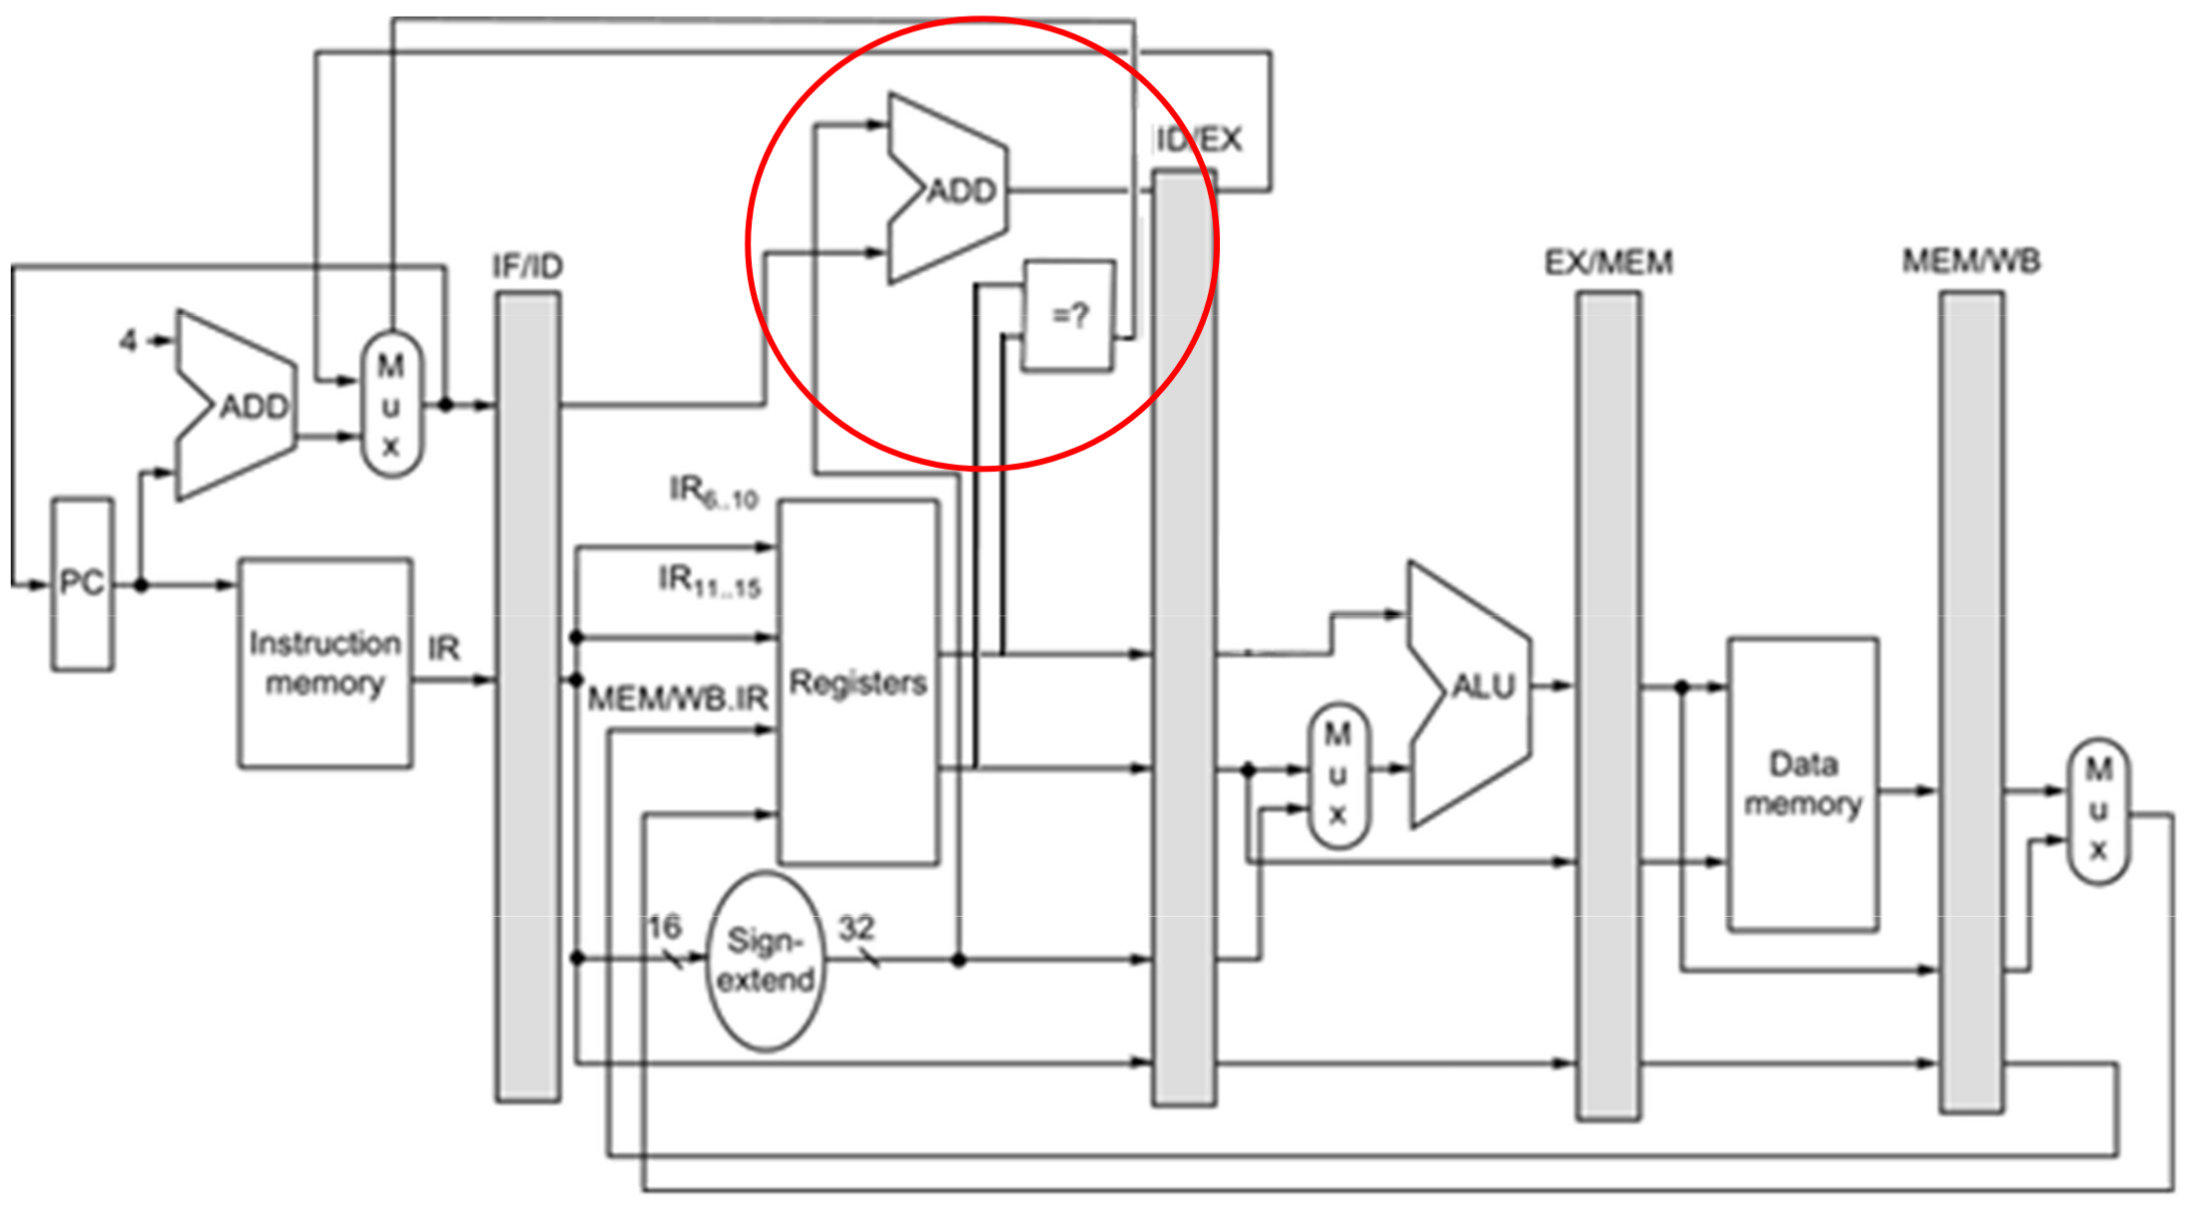
\includegraphics[scale=0.2]{../figures/modif_pipeline.png}
\end{center}

Note that this approach has an issue: at most we can put the branch prediction in the ID (decode) stage, that is the second stage of the branch instruction processing.
This means that the instruction loaded in the pipeline right after the branch one is always wasted (never depends on the branch prediction).

We show a figure that details this situation.
\begin{center}
	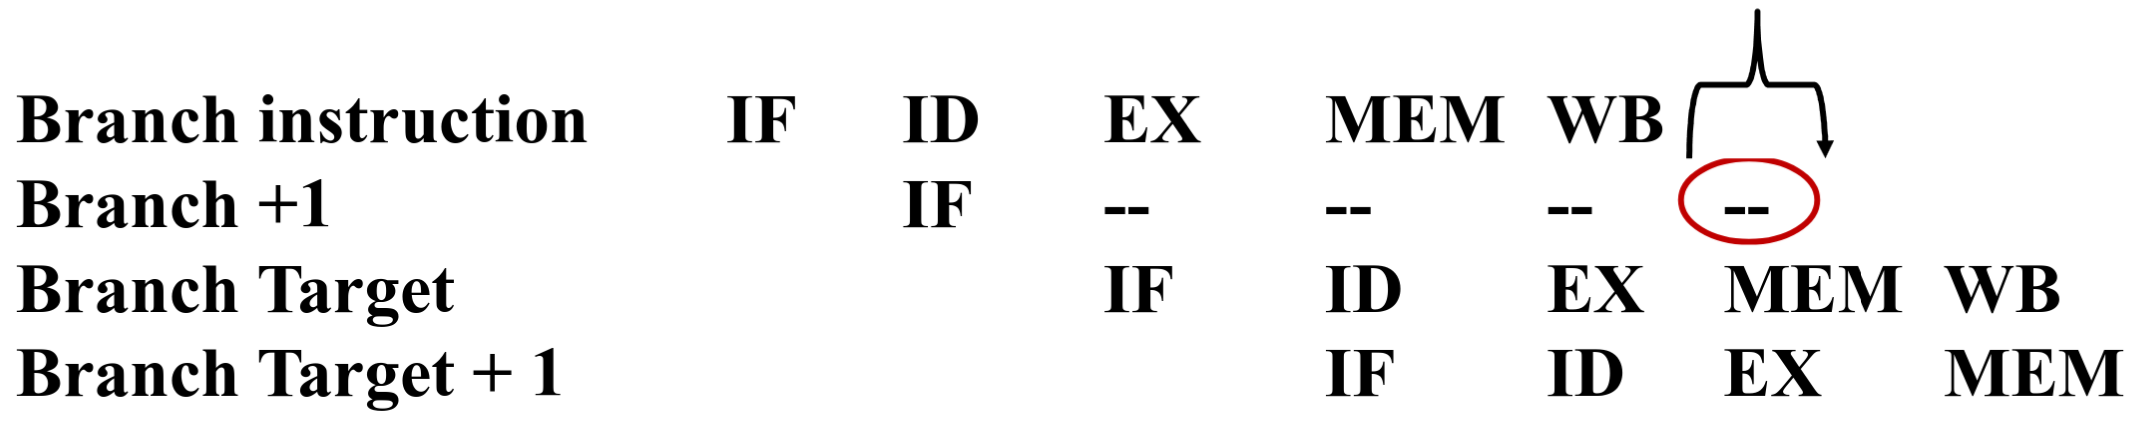
\includegraphics[scale=0.2]{../figures/bad_branch.png}
\end{center}

From this, we introduce the fact that several techniques can be used to manage branches:
\begin{itemize}
	\item Freezing the pipeline;
	\item Predict untaken;
	\item Predict taken;
	\item Delayed branch.
\end{itemize}

\subsubsection{Freezing the pipeline}

This is the previously proposed solution: the pipeline is stalled (or flushed) as soon as a branch instruction is detected, and until the decision about the branch is known.
It is the simplest solution to implement.

It wastes 2 clock cyceles (without the modified pipeline), or at least 1 (with the modified pipeline, decode is second stage).

\subsubsection{Predict untaken}

This technique introduces a \textit{guess}.
The \textit{predictions} we talked about so far weren't predictions in the strict sense: at most we were making the actual condition calculation earlier (in the ID stage), but we still were sure about actual branches taken.
Now we assume an arbitrary value of the condition before evaluating it:
\begin{itemize}
	\item We assume the branch is not taken;
	\item We avoid any change in the pipeline status until the branch decision has been taken;
	\item We undo all the performed operations if the branch turns out to be taken.
\end{itemize}

Considering our last solution, this makes the most sense as we loaded the instruction after the branch anyways: if the branch isn't taken, there's no point in flushing.

\begin{center}
	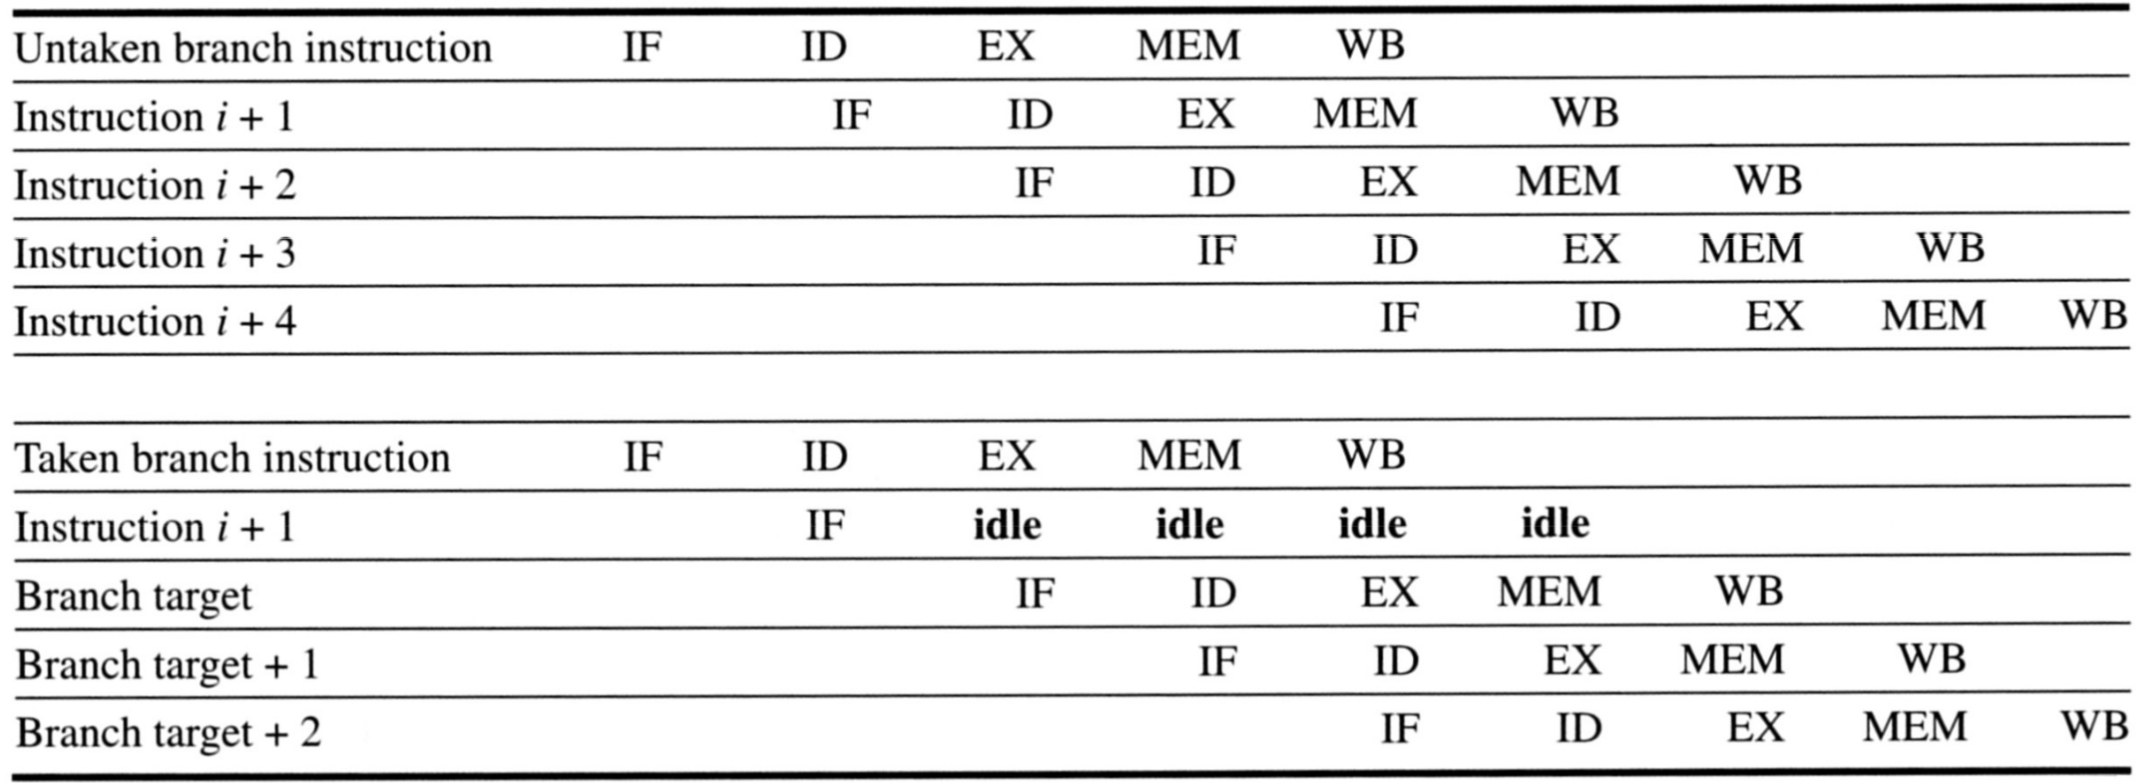
\includegraphics[scale=0.2]{../figures/pred_untaken.png}
\end{center}

\subsubsection{Predict taken}

The same technique can be done by \textit{guessing} the branch is taken.
The results are the same, just that we load the instruction after the target (instead of the one after the branch).
Performance gains are similar assuming branches get taken or not taken with equal probability.

\par\smallskip

Note the role of the \textit{compiler}:
If the hardware supports the predict taken or predict
untaken scheme, the compiler can improve performance
by generating code which maximizes the chance for the
processor to make the right prediction.

For instance:
considering the loop implementation, the for scheme is
suitable for the predict untaken scheme, the do while
for the predict taken.
In fact, the for scheme involves executing a conditional
branch instruction before the loop body, which results in
a not taken branch as many time as the number of
iterations. the do while does the opposite.

\subsubsection{Delayed branch}

This technique is based on filling the slot after the
branch instruction (named branch-delay slot) with
instructions which have to be executed no matter the
branch outcome.
It is an actual \textit{architectural} change on the ISA: branches actually branch only after one instruction, and the slot which was wasted before now has a fixed purpose.

It is up to the compiler (or the seasoned programmer) to fill each branch-delay slot with
the right instructions.
The processor does nothing special when a branch
instruction is decoded.

\begin{center}
	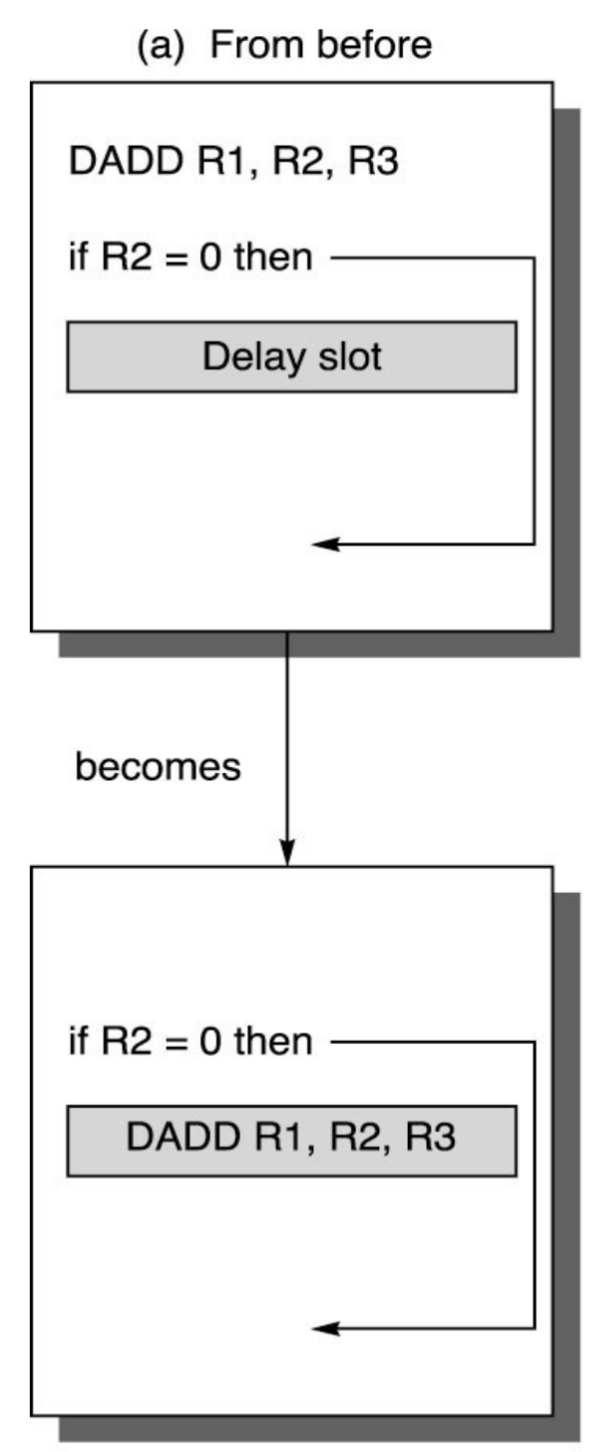
\includegraphics[scale=0.2]{../figures/delay_branch.png}
\end{center}

MIPS famously used one branch delay slot. ARM also historically had behavior resembling this in older ARM architectures, where instructions following a branch could already have entered the pipeline, but ARM's architectural rules are different from the classic MIPS "one guaranteed delay-slot instruction" model.
Today, other techniques are preferred.

The performance depends on the compiler ability in finding the right
instructions to put in the delay slots.
We find that using this technique, only about 30\% of branches do
produce a penalty.

When deeply pipelined processors are used, the delay
slots is longer, and the advantages of delayed-branches
smaller.
Therefore, such RISC architectures do not support
delayed branches.

\subsection{Multicycle operations}

Let's talk \textit{complex operations}, such as \textbf{floating point}.
Floating point units perform more complex operations than integer ones.
Therefore, in order to force them to perform their job in a single clock cycle, the designer should:
\begin{itemize}
	\item Either use a very slow clock;
	\item Or make these units very complex.
\end{itemize}
As a popular alternative, floating point units generally
require more than one clock cycle to complete.
The EX stage is composed of different functional units,
and takes as many clock cycles, as the instruction
requires.

\subsubsection{Multicycle execution}

The resulting pipeline is as follows, with the EX stage divided in multiple units with feedback and (possibly) multicycle instruction permanence.

\begin{center}
	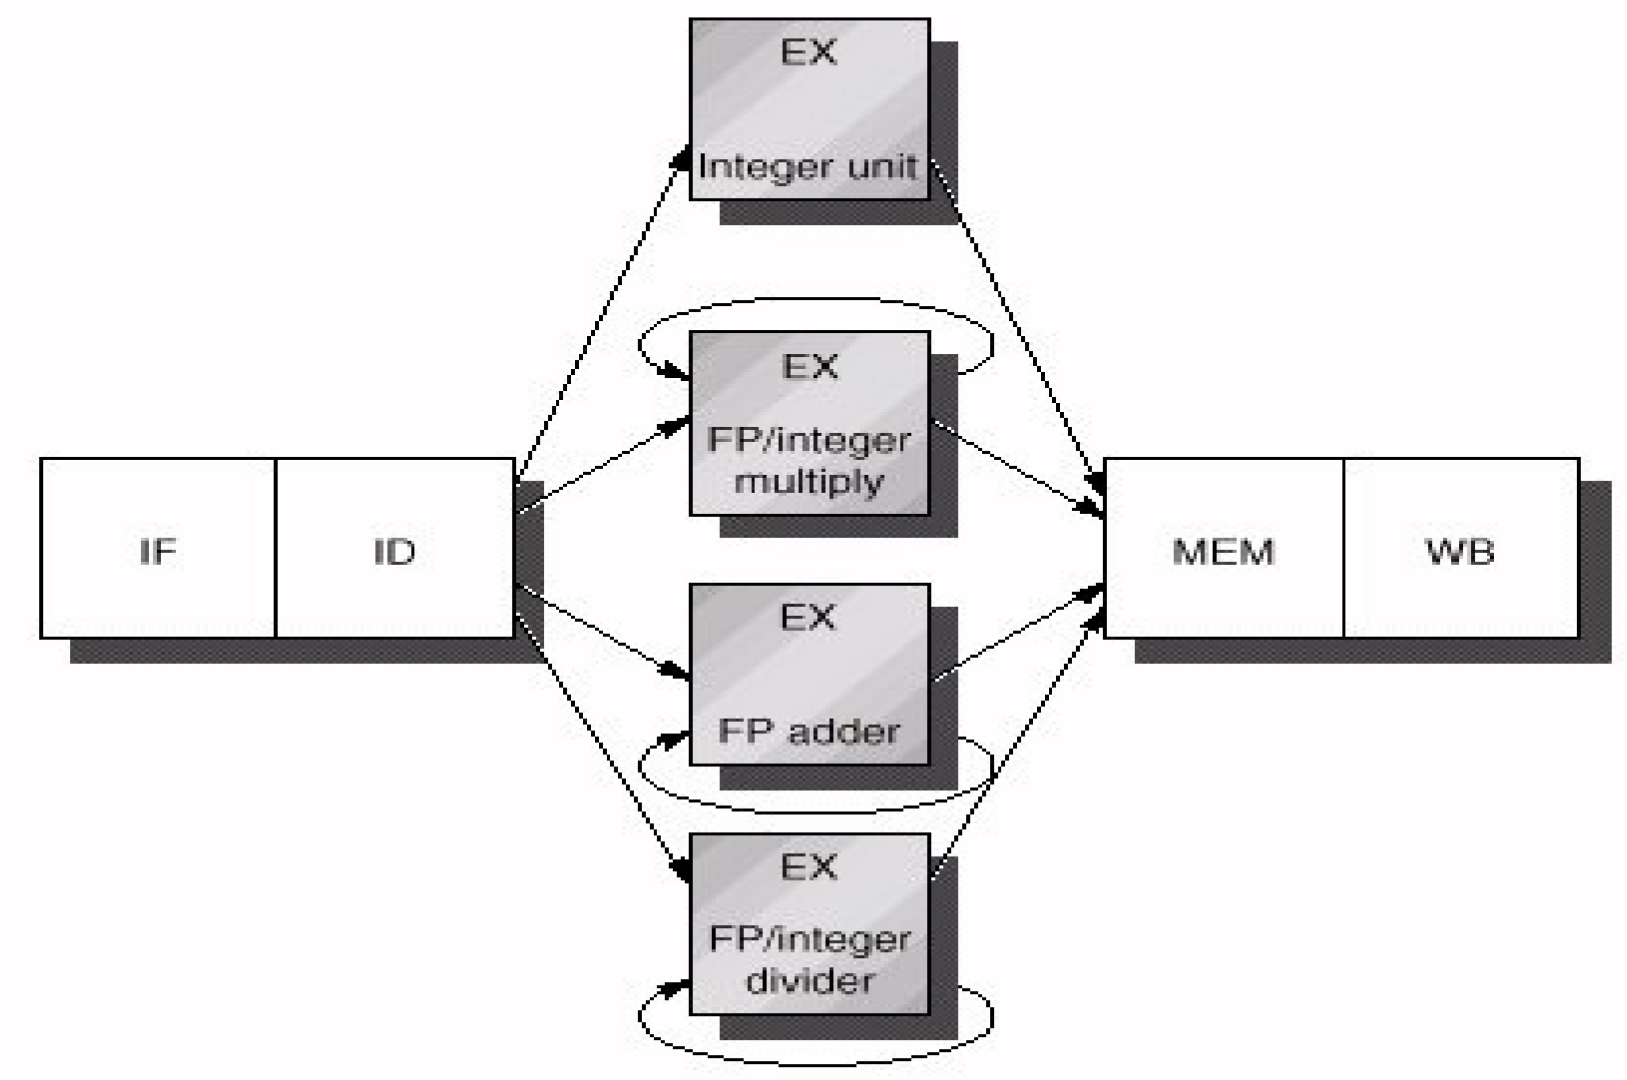
\includegraphics[scale=0.222]{../figures/fp_pipeline.png}
\end{center}

We see the problems of this approach by considering certain \textit{metrics} of the execution phase:
\begin{itemize}
	\item \textbf{Latency}: it is the number of cycles that should last
	      between an instruction that produces a result
	      and an instruction that uses the same result;
	\item \textbf{Initiation interval}: it is the number of cycles that must elapse
	      between issuing two operations of the same
	      type to the same unit.
\end{itemize}

This approach increases latency as some instructions stay in the execution stage longer.

\subsubsection{Multicycle pipelines}

An improvement is to \textit{pipeline} our expanded execution stage:

\begin{center}
	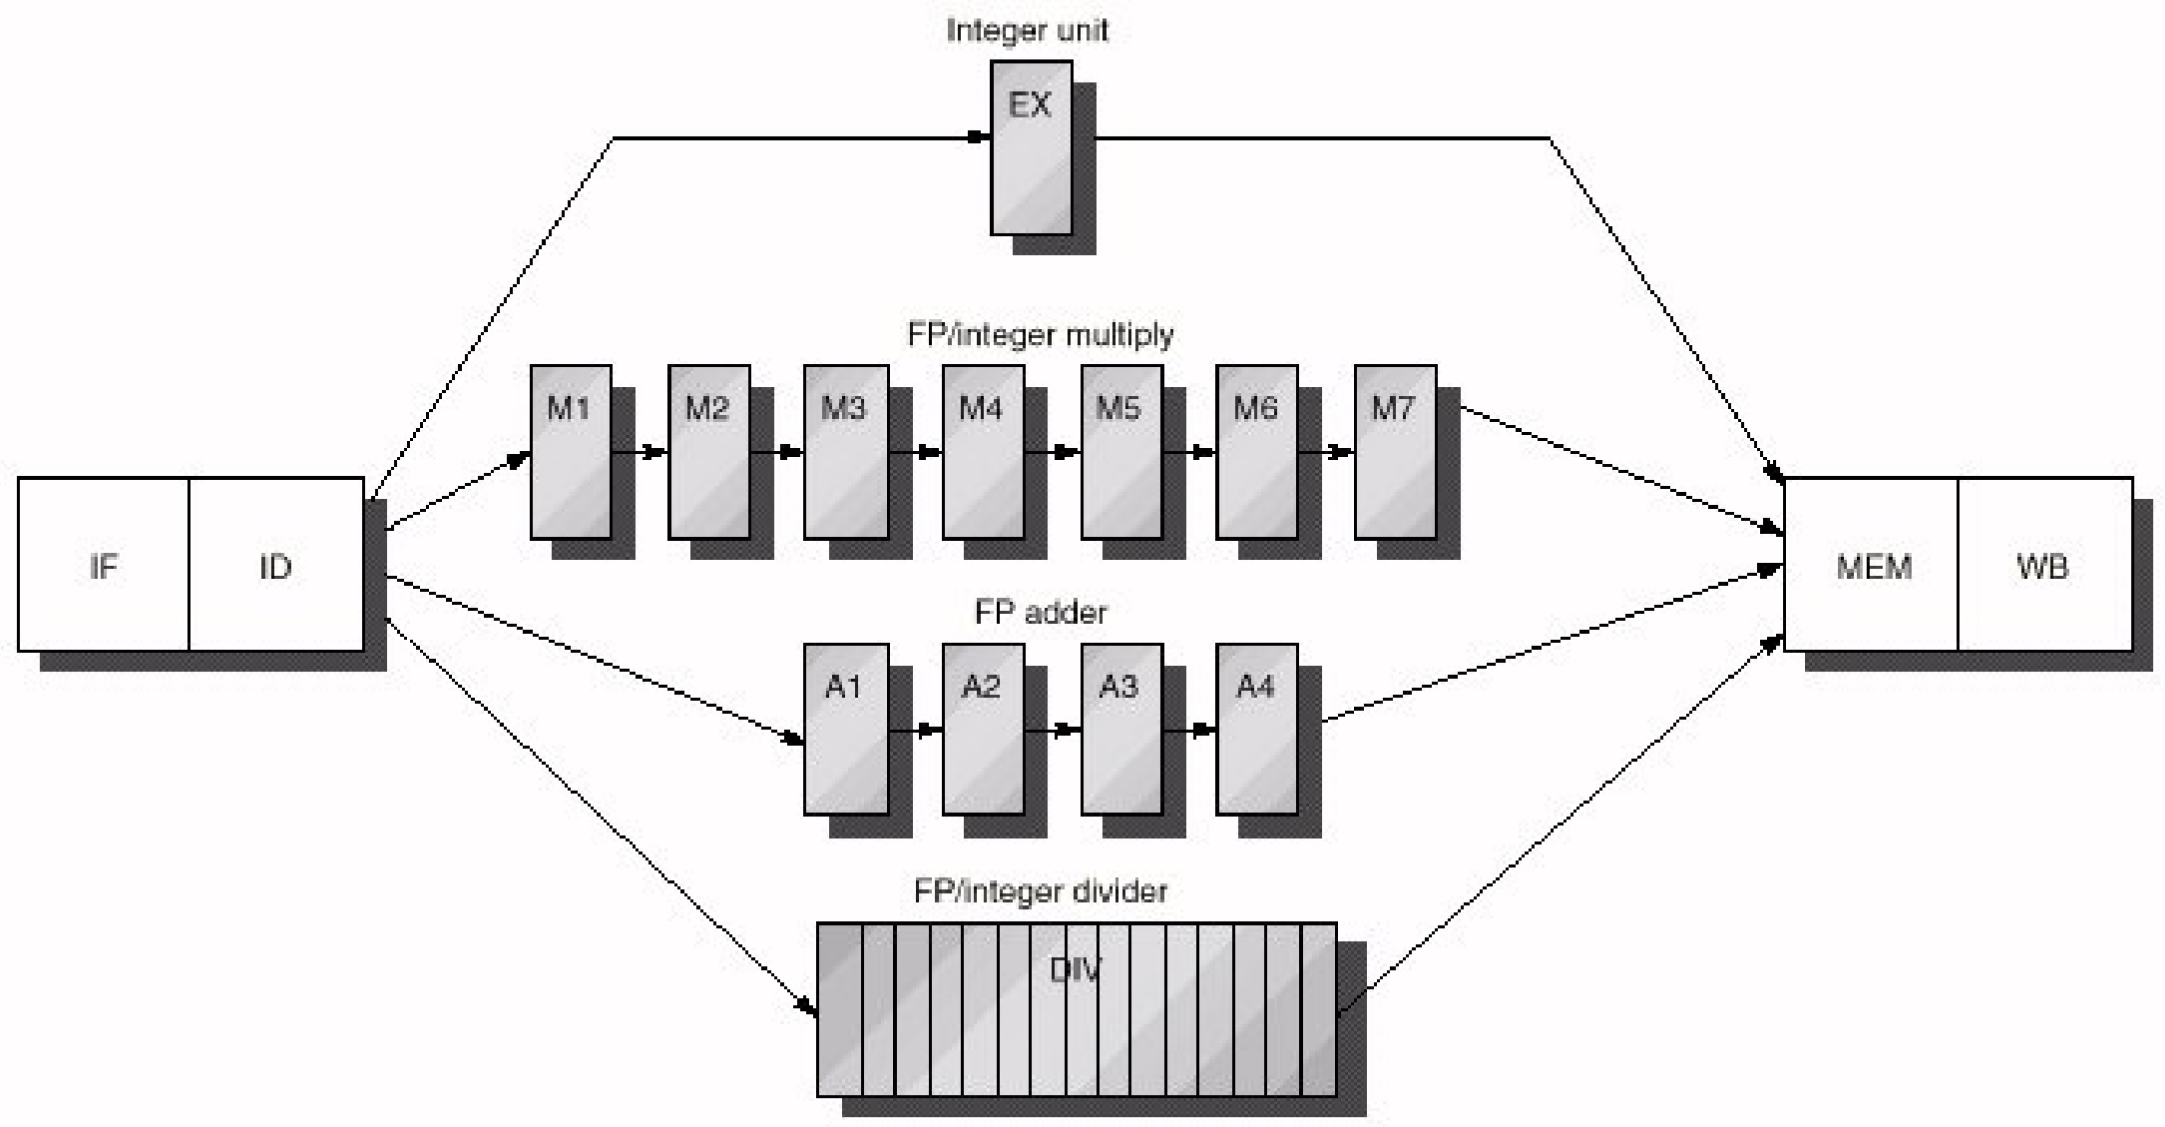
\includegraphics[scale=0.2]{../figures/fp_pipeline_1.png}
\end{center}

Each instruction, as with all pipelines, stays in the processor the same amount of time (if not longer because of pipelining overhead), but at least we have the increased throughput from more instruction coexisting in the pipeline at the same time.

One thing to note, though, is that due to the different structure of the EX stage, \textit{hazards} may become more frequent.

\subsubsection{Multicycle hazards}

Let's see the \textbf{hazards} we can encounter with this architecture.

\begin{itemize}
	\item \textbf{Structural hazards} can occur in ways we didn't encounter before:
	      \begin{itemize}
		      \item Because of the unpipelined divide unit (at least in our example above), several instructions could need it at the same time;
		      \item Because the instructions have varying running times, the number of register writes required in a cycle can be larger than 1 (and this applies generally).
		            \begin{center}
			            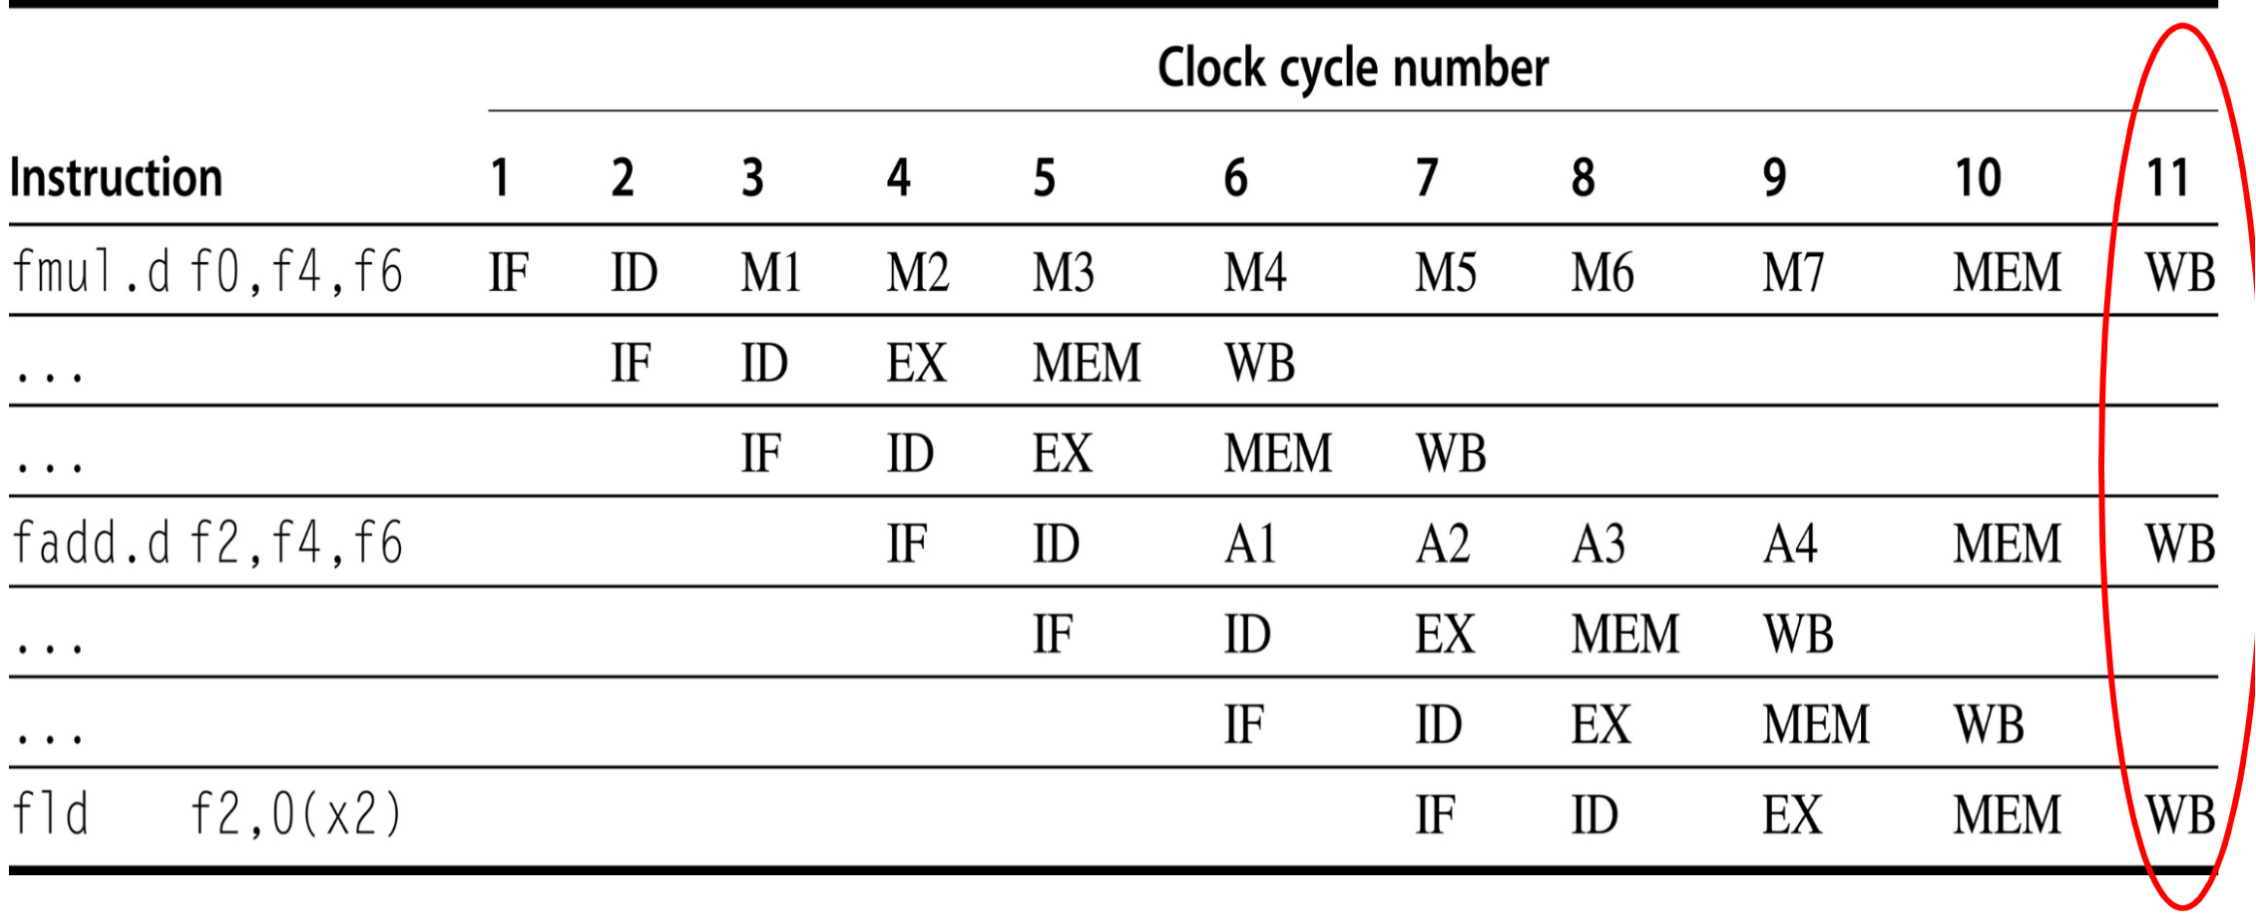
\includegraphics[scale=0.2]{../figures/multi_wb.png}
		            \end{center}
		            This is particularly bad as in our integer pipeline there was no way to have WB stages overlap.
	      \end{itemize}

	      The solutions, as always (we saw structural hazards on the integer pipeline), are:
	      \begin{itemize}
		      \item Adding other write ports (normally too expensive)
		      \item Forcing a structural hazard via \textit{stalling}:
		            \begin{itemize}
			            \item Instructions are stalled in the ID stage;
			            \item Or instructions are stalled before entering the MEM or WB stage.
		            \end{itemize}
	      \end{itemize}

	\item \textbf{Data hazards} can occur, are more frequent and have an higher performance impact.
	      \begin{itemize}
		      \item Because of longer latency of operations, stalls for data hazards may stall the pipeline for longer periods.

		            \begin{center}
			            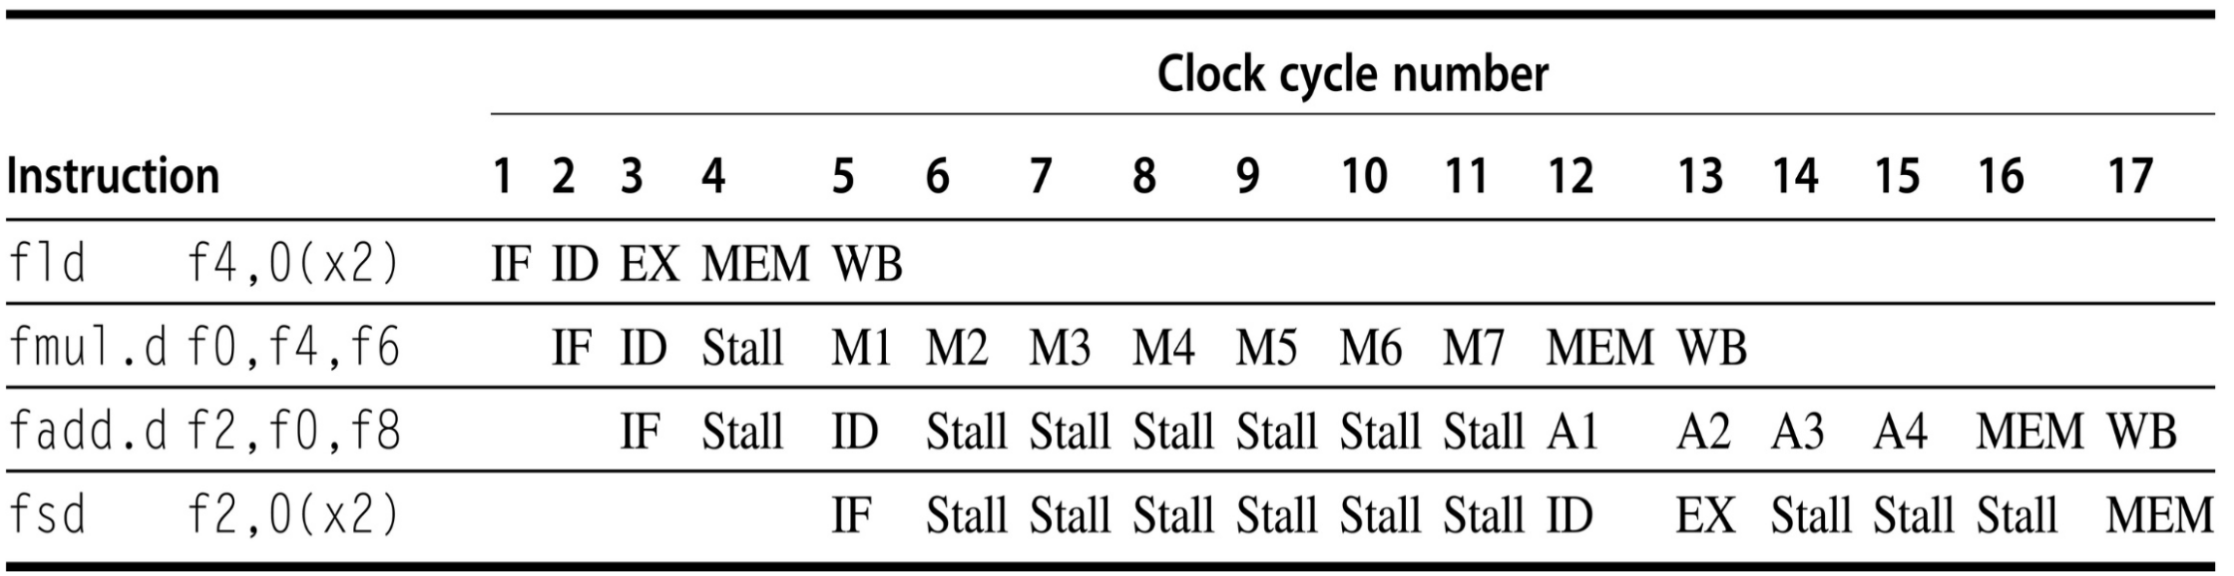
\includegraphics[scale=0.2]{../figures/big_dhazard.png}
		            \end{center}

		            As with the before example, the long stall is due to the hefty execution size of the floating point instructions, which keeps the target register "locked" for more than our integer pipeline did.

		            This is a case of a \textbf{RAW} (\textit{Read After Write}) hazard;

		      \item The concurrent WB retires are also worth noting: new kinds of data hazards might manifest because multiple instructions reach WB at the same time.

		            This is a case of a \textbf{WAW} (\textit{Write After Write}) hazard.

		            The simple solution is: before issuing an instruction to the EXE stage, check
		            whether it is going to write on the same register of an
		            instruction still in the EXE stage.
		            In this case, stall the new instruction.
	      \end{itemize}

\end{itemize}

\subsubsection{Summary of hazards}

To sumamrize, iif hazard detection is always performed in the ID stage,
three checks have to be performed:
\begin{itemize}
	\item Structural hazards (involving the divide unit and the write port);
	\item RAW data hazards: check whether some source
	      register is listed among the destination registers of
	      pending instructions, and whether this register will
	      not be available at the right moment
	\item WAW data hazards: check whether the instruction
	      currently in ID has the same destination register of
	      any instruction in EXE.
\end{itemize}

\end{document}
